A potentially large problem with the application of the logistic model to antibody data is that low antibody titres do not necessarily correlate with a high probability of infection (which is one of the model's assumptions). This assumption of baseline risk of 1 can be justified if it is the case that subjects with low antibody titres always (or almost always) get infected. If a large proportion of subjects with low titres do not get infected, this assumption is not justified and this model will produce a poor fit. 

If the baseline risk cannot justifiably be assumed to be 1, the fitted probability curve will be flatter than the true curve, thereby misrepresenting the true probability of infection across the titre range as depicted in Figure \ref{LogisticFit}. Thus, ignoring the baseline risk assumption will lead to poor model fit and hence biased estimates of titre effect.

\begin{figure}[htp]
	\centering
	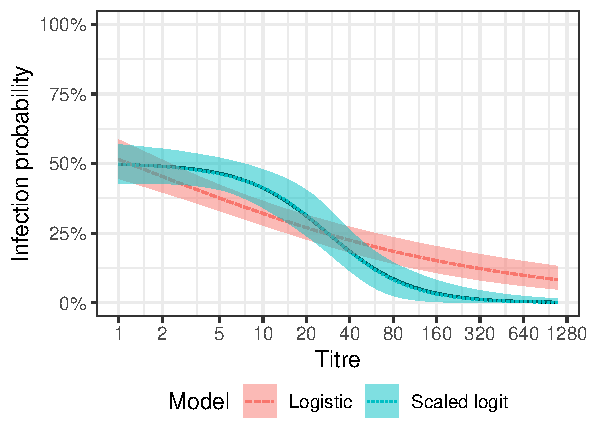
\includegraphics[width=0.6\textwidth]{../logistic-plot/predsplot.pdf}
	\caption{
	An illustration of a bad fit of the logistic model. The solid line ($0.5\frac{\text{exp}(5 - 1.5 X_{\text{logtitre}})}{1 + \text{exp}(5 - 1.5 X_{\text{logtitre}})}$) is the true probability curve where the baseline risk is 0.5. The dashed line is the expected fitted probability curve from standard logistic regression. The dotted line is the fitted probability curve from scaled logistic regression. The shaded regions are the 95\% confidence intervals. The expected curves and CIs was obtained from 10,000 simulations each with 500 observations simulated from the true curve. The models were fitted to each simulated dataset and the means of the regression estimates were taken from all simulations.
}
	\label{LogisticFit}
\end{figure}

Estimating the baseline risk in the above model leads to the scaled logit model.
